
\subsubsection{01.10.14}

\begin{enumerate}
	\item Время начала и окончания собрания:
	18:00 - 21:30
	\item Цели собрания:
	\begin{enumerate}
		\item Выбрать и сделать колесную базу робота.
		
		\item Создать простейшую программу для управления им с джойстика.
		
	\end{enumerate}
	
	\item Проделанная работа:
	\begin{enumerate}
		\item Была создана колесная база робота:
		\begin{enumerate}
			\item Предпочтение было отдано варианту с омни-колесами с роликами, расположенными под углом в 45 градусов к направлению вращения, однако, поскольку пока у нас в наличии их не было, вместо омни-колес было решено установить обычные колеса из набора TETRIX.
			
			\item Для обеспечения устойчивости робота наиболее тяжелые компоненты были расположены как можно ближе к земле. Таким образом, в нижней части робота был расположен аккумулятор (он, как самая тяжелая деталь робота, был помещен в заднюю часть для того, чтобы уравновесить захват мячей, который будет располагаться в передней части робота), микроконтроллер NXT и драйвера моторов и сервоприводов.
			
			\item Поскольку вся управляющая электроника была размещена у самого пола, провода могли случайно вылезти наружу с нижней части и зацепиться за других роботов или за собственные подвижные части, поэтому на следующее занятие было решено принести пластмассовую папку и вырезать из нее кусок для днища нужного размера, чтобы защитить управляющую электронику с проводами с нижней части.
			
			\begin{figure}[H]
				\begin{minipage}[h]{0.2\linewidth}
					\center  
				\end{minipage}
				\begin{minipage}[h]{0.6\linewidth}
					\center{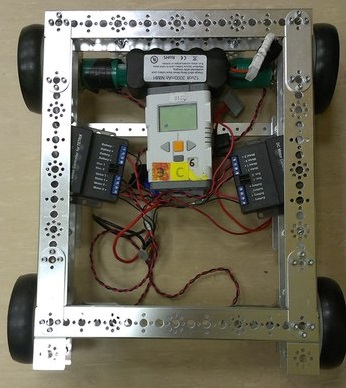
\includegraphics[scale=0.5]{days/01.10.14/images/01}}
					\caption{Колесная база робота}
				\end{minipage}
			\end{figure}
			
		\end{enumerate}
		
		\item Была выдвинута идея сделать подъемник для мячей по принципу конвейера. Такая система позволила бы установить захват мячей стационарно на корпусе робота, а поднимать только сами мячи. Вот идеи конвейеров:
		\begin{enumerate}
			\item Лента с корзинами, расположенными на ней через равные промежутки.
			
			\item Раздвижной полый цилиндр, внутри которого перемещаются оси, выполняющие роли основания корзины, стенками которой являются стенки раздвижного цилиндра.
			
			\item Раздвижной полый цилиндр, внутри которого с одной стороны расположена движущаяся вверх лента с закрепленными на ней упругими «ворсинками», проталкивающими шары вверх по трубе. Плюс данной системы в том, что мячи могут захватываться лентой сразу, а не ждать следующую корзину.
			
			\begin{figure}[H]
				\begin{minipage}[h]{0.2\linewidth}
					\center  
				\end{minipage}
				\begin{minipage}[h]{0.6\linewidth}
					\center{
\includegraphics[scale=0.25]{days/01.10.14/images/02}}
					\caption{Идеи для подъемника мячей: 1)Лента с корзинами 2)Конструкция с раздвижным цилиндром 3)Конструкция с раздвижным цилиндром и ворсинками}
				\end{minipage}
			\end{figure}
			
		\end{enumerate}
		
	\end{enumerate}
	
	\item Итоги собрания: 
	\begin{enumerate}
		\item Колесная база робота собрана.
		
		\item Программа управления роботом не реализована.
		
	\end{enumerate}
	
	\item Задачи для последующих собраний:
	\begin{enumerate}
		\item Создать программу управления роботом.
		
		\item Установить защиту днища.
		
	\end{enumerate}     
\end{enumerate}
\fillpage

